\documentclass[12pt,a4paper]{article}
\usepackage{amsmath}
\usepackage{amssymb}
\usepackage{graphicx}
\usepackage{tabularx}
\usepackage{diagbox}
\usepackage{geometry}
\usepackage{cite}
\usepackage{bm}
\usepackage{algorithm}
\usepackage{algpseudocode} 
\usepackage{enumitem}
\usepackage{verbatim}
\usepackage{color,xcolor}
\newgeometry{left=1.8cm,right=1.8cm,top=2cm,bottom=2cm}
\title{IE 56100 Final Project Proposal}
\author{Qinbo Bai, Kun Qian}
\date{Nov. 4, 2019}
\usepackage[round]{natbib}
\renewcommand{\bibname}{References}
\renewcommand{\bibsection}{\subsubsection*{\bibname}}
\begin{document}
	\maketitle
	\section{Introduction of the topic}
	\noindent
	\par As the deep learning technology becomes popular, it has been successfully applied to many fields. In recent years, it has been considered in the physical layer of communication system. Different from the traditional communication system, which consists of several blocks to finish the communication task, end-to-end communication system has been fulfilled by deep learning and achieve similar performance. Fig. \ref{end2end} gives the concept of such a system.
	\begin{figure}[h] \label{end2end}
		\centering
		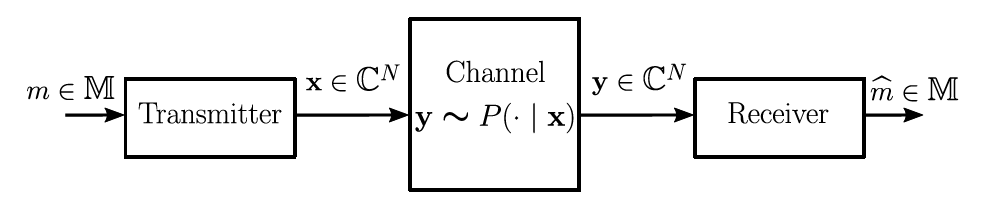
\includegraphics[width=3.5in]{end2end.png}
		\caption{The architecture of end-to-end communication system}
	\end{figure}
	\par Using deep learning technology, we implement both the transmitter and receiver as the neural network and interpret the whole system as an autoencoder. In order to optimize the whole system, we need to do the back-propitiation with respect to transmitter and receiver. However, without the exact formulation of channel function, the optimization for transmitter cannot be implemented directly, and the project aims to optimize the whole system with zero-order information.
	\section{Problem formulation}
	\noindent
	\par  An end-to-end communication system is designed to reliably exchange message at two nodes. The transmitter maps a message $\bm{s}$ from the set $\mathbf{S}={1,2,...,s}$ to a $N$ dimensional complex number $\bm{x}$. At the receiver, a distorted symbol $\hat{\bm{x}}$ is received due to the impairments of the channel. Finally, the receiver maps the distorted symbol $\hat{\bm{x}}$ to the estimated $\hat{\bm{s}}$. The goal of a successful system is to establish the faithful reconstruction.
	\par To make the following statement clear, we denote the transmitter and receiver as function $f_T$ and $f_R$ with the parameter $\bm{\theta_T}$ and $\bm{\theta_R}$ in the neural network. Furthermore, we denote the channel as function $h$ with some parameter $\bm{\theta_H}$. Thus, the restored symbol can be express as:
	\begin{equation}
		\begin{aligned}
			\hat{\bm{s}}=f_R(h(f_T(\bm{s},\bm{\theta_T}),\bm{\theta_H}),\bm{\theta_R})
		\end{aligned}
	\end{equation}
	\par In order to optimize the parameter in the transmitter and receiver, a loss function between $\bm{s}$ and $\hat{\bm{s}}$ needs to be established. A common choice is the cross-entropy function, and the per-example loss is as below:
	\begin{equation}
		l^{i}=\sum_{s_j\in\bm{s}_i}-s_j\log(\hat{s_j})
	\end{equation}
	\par The total loss is the sum of loss over $M$ symbols:
	\begin{equation} \label{loss}
		\mathcal{L}(\bm{s}_{1:M},\hat{\bm{s}_{1:M}})=\sum_{i=1}^{M}l^i=\sum_{i=1}^{M}\sum_{s_j\in\bm{s_i}}-s_j\log(\hat{s_j})
	\end{equation}
	
	{\color{blue}
	\par Thus, our optimization problem without constrain can be express as:
	\begin{equation}
	\min\limits_{\bm{\theta_T},\bm{\theta_R}}\mathcal{L}(\bm{s}_{1:M},\hat{\bm{s}_{1:M}})
	\end{equation}
	}
	\par Using the gradient descent algorithm, we do back-propagation on $\hat{\bm{s}}$ with respect to $\bm{\theta_T}$ and $\bm{\theta_R}$. Receiver optimization is trivial. However, based on the chain rule,
	\begin{equation}
		\frac{\partial\mathcal{L}}{\partial\bm{\theta_T}}=\frac{\partial\mathcal{L}}{\partial f_R}\cdot\frac{\partial f_R}{\partial h}\cdot\frac{\partial h}{\partial f_T}\cdot\frac{\partial f_T}{\partial\bm{\theta_T}}
	\end{equation}
	\par Without the knowledge of function $h$, this cannot be calculated directly. {\color{blue} Thus, our problem is how optimize the communication system without the exact form of the channel function. In other other, optimize the communication system in zeroth-order oracle.}
	\section{Training Transmitter with Reinforcement Learning}
	\noindent
	\par \citep{8645416} uses the reinforcement learning to train the transmitter without using the knowledge of channel function. The implement is shown in Fig. \ref{RL}. 
	\begin{figure}[h] \label{RL}
		\centering
		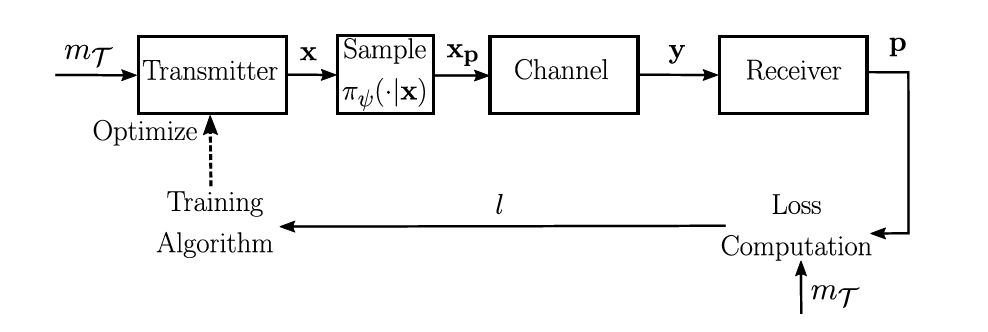
\includegraphics[width=3.5in]{RL.png}
		\caption{RL approach to train the transmitter}
	\end{figure}
	\par In order to enable the exploration, the author maps the output of the transmitter $\bm{x}$ to the random variable $\bm{x}_p$ with Gaussian distribution. It means,
	\begin{equation}
		\bm{x}_p=\sqrt{1-\sigma^2}\bm{x}+\bm{\omega}
	\end{equation}
	\par where $\omega$ is a complex gaussian random vector with $\bm{\omega}\sim\mathcal{CN}(\bm{0},\sigma^2\mathbf{I})$. Obviously, the pdf of $\bm{x}_p$ can be expressed as:
	\begin{equation} \label{policy}
		\pi(\bm{x}_p\vert f_{\theta_T}(s))=\frac{1}{(\pi\sigma^2)^N}\exp(-\frac{\Vert\bm{x}_p-\sqrt{1-\sigma^2}f_{\theta_T}(s)\Vert^2}{\sigma^2})
	\end{equation}
	\par To see how to modify this problem to a RL problem, we regard the message $s$ as the state, the input of channel $\bm{x}_p$ as the action, the per-example loss $l$ as the cost. The policy is the action distribution given the state, which is the Gaussian policy shown exactly by equation Eq. \eqref{policy}. It is obvious that the next state(next message) is independent of the current state(current message) and current action(current input of the channel). Thus, we can consider each episode of the reinforcement learning as 1. 
	\par Using the Monte-Carlo simulation and famous policy gradient algorithm \citep{Sutton1998}, the parameter in transmitter can be updated by
	\begin{equation}
		\bm{\theta_{T+1}}=\bm{\theta_T}-\eta\frac{1}{B_T}\sum_{i=1}^{B_T}l^{i}\nabla_{\bm{\theta}_T}\log(\pi(\bm{x}_p^{i}\vert f_{\bm{\theta}_T}(s^{i})))
	\end{equation}
	\par where the gradient in the above equation can be computed as below,
	\begin{equation}
		\nabla_{\bm{\theta_T}}\log(\pi(\bm{x}_p\vert f_{\bm{\theta_T}}(s^i)))=\frac{2\sqrt{1-\sigma^2}}{\sigma^2}\big(\nabla_{\bm{\theta}_T}f_{\bm{\theta}_T}(s^i)\big)^T\big(\bm{x}_p-\sqrt{1-\sigma^2}f_{\bm{\theta}_T}(s^i)\big)
	\end{equation}
	\par In order to implement RL algorithm, it is convenient to use popular deep learning platform such as \textbf{Tensor-flow} to run auto-gradient.
	\section{Training Transmitter with direct non-convex zeroth-order optimization}
	\noindent
	\par Based on \cite{jin2017escape} work, I purpose a zeroth-order algorithm \citep{2019arXiv191001277B} to direct optimization the function with only the access to the function value, which means the exact form of the channel function isn't needed anymore. The basic idea of this algorithm is to split the optimization into two parts. Firstly, we need to use the function evaluation to estimate the gradient at a given point. Then, follow the framework of \cite{jin2017escape} algorithm to finish the gradient descent. Next, we show the algorithm to estimate the gradient.
	\begin{algorithm}[h]
		\label{GE}
		\caption{Gradient Estimation $GE({d,l,B,c',\hat{\epsilon},\bm{x}})$}
		\begin{algorithmic}[1]
			\State $v\leftarrow\frac{\hat{\epsilon}}{c'l(d+3)^{1.5}}$, $\sigma^2\leftarrow2c'^{2}(d+4)B^2$, $m\leftarrow\frac{32\sigma^2}{\hat{\epsilon}^2}(\log(\frac{1}{\hat{\epsilon}})+\frac{1}{4})$
			\State Generate $\bm{u}_1,...\bm{u}_m$, where $\bm{u}_i\sim\mathcal{N}(0,\mathbf{I}_d)$
			\State $\hat{\nabla}f(\bm{x})=\frac{1}{m}\sum_{i=1}^{m}\frac{f(\bm{x}+v\bm{u}_i)-f(\bm{x})}{v}\bm{u}_i$ 
			\State \Return $\hat{\nabla}f(\bm{x})$
		\end{algorithmic}
	\end{algorithm}
	\par Consider the whole cost function as $f$ with variable $\bm{\theta}_T$. Algorithm  \ref{GE} gives the approach to estimate the gradient with the method of Gaussian smoothing. $d$ is the dimension of $\bm{\theta}_T$,  $l$ is $l$-smooth parameter of function $f$, $B$ is the bound for gradient norm $\Vert \nabla f\Vert$, $c'>1$ is a constant. $\bm{x}$ is the point we make an estimation and $\hat{\epsilon}$ is the intended gap between the estimated gradient and true gradient. The line 1 in the algorithm gives the parameter used in the following lines. $v$ is the Gaussian smoothening parameter. $\sigma^2$ is the bound for the variance of gradient estimator in one sample. $m$ gives the total number of samples we need to get error less than $\hat{\epsilon}$. Line 2 generates $m$ Gaussian random vector with zero mean and variance $\mathbf{I}_d$ which are used to calculate the estimate of the gradient. The estimation algorithm (Line 3) takes an average of estimated gradient using $m$ samples. 
	\par Next algorithm utilizes the estimated gradient and optimize the transmitter.
	\begin{algorithm}[h]
		\label{PGD-MF}
		\caption{Estimated Gradient Descent Algorithm $EGD(\bm{x}_0,d,l,B,\chi_1,\theta,\rho,\epsilon,\hat{\epsilon},c,c',\delta,\Delta_f)$}
		\begin{algorithmic}[1]
			\State $\chi \leftarrow \max\{(1+\theta)\log(\frac{2d\ell\Delta_f}{c\epsilon^2\delta}), \chi_1\}$, $\eta\leftarrow\frac{c}{l}$, $g_{thres}\leftarrow\frac{\sqrt{c}}{\chi^2}\cdot\epsilon$, $f_{thres}\leftarrow\frac{c}{\chi^3}\cdot\sqrt{\frac{\epsilon^3}{\rho}}$, $t_{thres}\leftarrow\frac{\chi}{c^2}\cdot\frac{l}{\sqrt{\rho\epsilon}}$, $t_{temp}\leftarrow-t_{thres}-1$, $r\leftarrow \frac{g_{thres}}{l}$
			\For{$t=0,1,...$}
			\State $\hat{\nabla}f(\bm{x}_t)=GE(d,l,B,c',\hat{\epsilon},\bm{x}_t)$
			\If{$\Vert\hat{\nabla}f(\bm{x}_{t})\Vert\leq g_{thres}$, $t-t_{temp}>t_{thres}$}
			\State $\bm{x}_t\leftarrow\bm{x}_t+\bm{\xi}_t$, $\bm{\xi}_t\sim\mathbb{B}_{\bm{x}_t}(r)$
			\State $t_{temp}\leftarrow t$
			\EndIf
			\If{$t-t_{temp}=t_{thres}$ and  $f(\bm{x}_t)-f(\bm{x}_{t-t_{thres}})>-f_{thres}$}
			\State \Return $\bm{x}_{t-t_{thres}}$
			\EndIf
			\State $\bm{x}_{t+1}\leftarrow\bm{x}_t-\eta\hat{\nabla}f(\bm{x}_t)$
			\EndFor
		\end{algorithmic}
	\end{algorithm}
	\par It can be proved that the final output of the algorithm is an second-order $\epsilon$ stationary point. Thus, it can be the local minimal of the function $f$ (escape all strict saddle point). 
	\section{Final project plan}
	\noindent
	\par The plan of this project is to implement the two methods given in section 3 and 4, compare the performance and convergence rate of these two approaches. Besides, the project will include the formal problem formulation, the analysis of problem properties, theoretical analysis of the proposed algorithm.
	\bibliographystyle{apalike}	
	\bibliography{ref}
\end{document}